\documentclass[compress]{beamer}

\usetheme{Luebeck}
\usepackage[utf8]{inputenc}
\usepackage{subfig}
\usepackage{utopia} %font utopia imported
\usepackage{arabtex}
\usepackage{utf8}
\setcode{utf8}
\usepackage{amsmath}
\usepackage{amssymb}
\usepackage{amsthm}
\usefonttheme{professionalfonts} % using non standard fonts for beamer
\definecolor{foo}{RGB}{106,141,143}
\usecolortheme[named=foo]{structure}
\setbeamercolor{subsection in head/foot}{bg=foo!80!black}
% This block of code defines the information to appear in the
% title page

\title[Introduction to ASIC Design] %optional
{ASIC Design Flow}

\subtitle{How to design your own chip}

\author[Ahmed Abdelazeem] % (optional)
{Ahmed Abdelazeem}
%{A.~B.~Arthur\inst{1} \and J.~Doe\inst{2}}

\institute[ZU] % (optional)
{
	Faculty of Engineering\\
	Zagazig University
}
%{
	%	\inst{1}%
	%	Faculty of Engineering\\
	%	Zagazig University
	%	\and
	%	\inst{2}%
	%	Faculty of Chemistry\\
	%	Very Famous University
	%}

\date[ZU 2023] % (optional)
{RTL2GDSII Flow, February 2022}

%\logo{
\includegraphics[height=1.5cm]{lion-logo.png}}

%End of title page configuration block
%------------------------------------------------------------

%------------------------------------------------------------
%The next block of commands puts the table of contents at the
%beginning of each section and highlights the current section:
\setcounter{tocdepth}{1} %%%
\AtBeginSection[]
{
	\begin{frame}
		\frametitle{Table of Contents}
		\tableofcontents[currentsection]
	\end{frame}
}
%------------------------------------------------------------


\begin{document}
	
	%The next statement creates the title page.
	\frame{\titlepage}
	
	
	%---------------------------------------------------------
	%This block of code is for the table of contents after
	%the title page
	\begin{frame}
		\frametitle{Table of Contents}
		\tableofcontents
	\end{frame}
	%---------------------------------------------------------
\section[Intro]{Introduction}
\subsection[Design]{VLSI Design Cycle}
\begin{frame}
	\frametitle{The Life of a CMOS Inverter}
	\begin{center}
		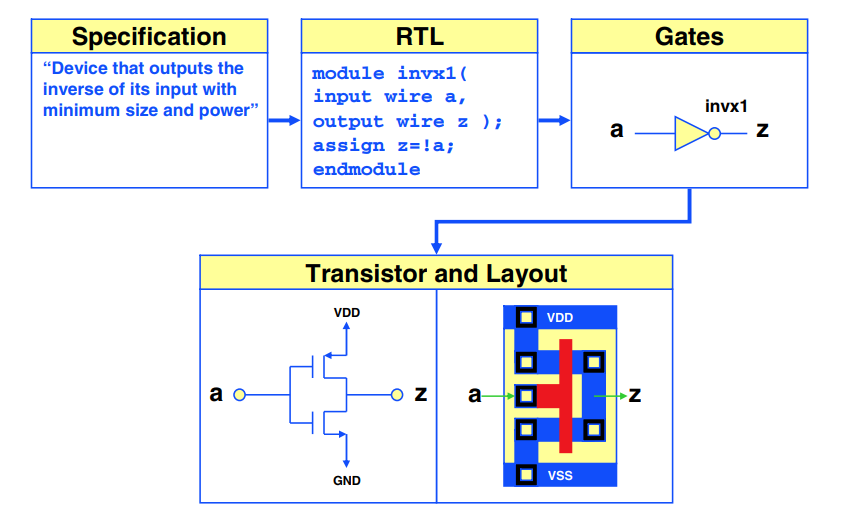
\includegraphics[width=\textwidth]{CMOS_CYCLE}
	\end{center}
\end{frame}	


\begin{frame}
	\frametitle{Design Implementation Flow}
	Much like the simple CMOS inverter, the general process of digital design implementation is the transformation of a design into various representations,eventually into physical hardware devices, just on a much BIGGER scale.
	\begin{center}
		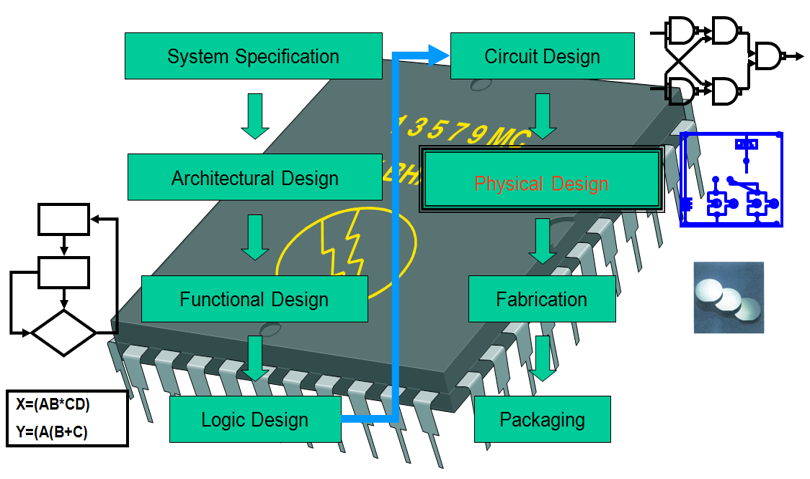
\includegraphics[width=0.8\textwidth]{design}
	\end{center}
	
\end{frame} 
\subsection[What]{What is Hardware Design ?}
\begin{frame}
	\frametitle{What is Hardware Design ?}
		Physically implementing an idea, a function, a system in hardware.
		\pause%
		\begin{block}{Find the optimal balance between:}
			\begin{itemize}
				\item Cost / Area
				\item Speed / Throughput
				\item Energy Consumption / Power Density
				\item Design Time
			\end{itemize}
		\end{block}
\end{frame}

\subsection[Tradeoffs]{Trade-offs in Design}
\begin{frame}
	\frametitle{Trade-offs in Design}
	\begin{block}{No free lunch}
	Depending on the design, some parameters are more important.
	You can generally sacrifice one parameter to improve the other:
	\pause%
	\begin{itemize}
		\item \textbf{Speed vs Area} \newline
			It is possible to speed up a circuit by using larger transistors,
			parallel computation blocks
			\pause
		\item \textbf{Design time vs Performance}
		\newline
		Given enough time, the circuits can be optimized for higher
		performance
	\end{itemize}
	\end{block}	
\end{frame}
\subsection[Examples]{Different designs, different requirements}
\begin{frame}
	\frametitle{What is Important for the Following Designs ?}
		\begin{center}
		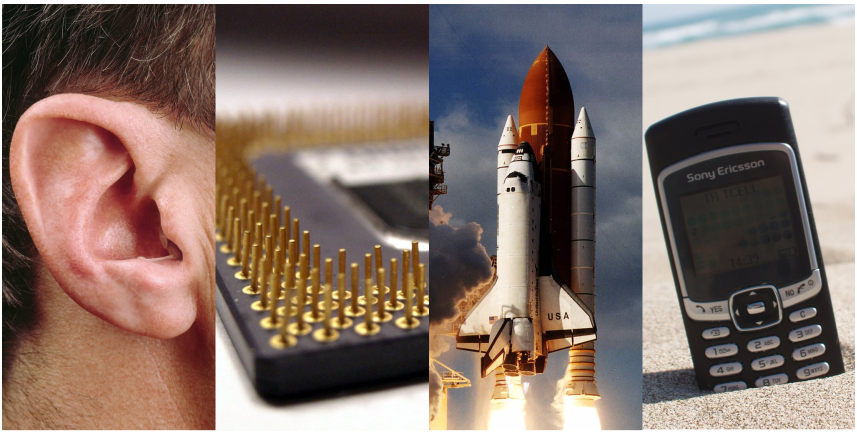
\includegraphics[width=\textwidth]{Examples}
	\end{center}
\end{frame}

\subsection[ASICs]{When to use use ASICs}
	\begin{frame}
		\frametitle{Application Specific Integrated Circuits}
				
\begin{columns}	
	\column{0.7\textwidth}
	\begin{center}
		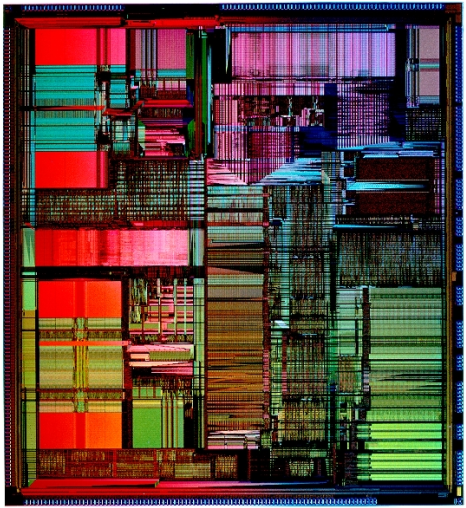
\includegraphics[width=0.7 \textwidth]{ASICs}
	\end{center}
	\column{0.53\textheight}
	\begin{block}{When to use ASICs ?}
		The good:
		\begin{itemize}
			\item Highest performance
			\item Cheap for mass production
		\end{itemize}
		The bad:	
		\begin{itemize}
			\item Long development time
			\item Not very configurable
			\item Requires specialization
		\end{itemize}
	\end{block}	
\end{columns}
	\end{frame}
\section[Flow]{Overall Design Flow}
\subsection[flow]{Overall Design Flow}
\begin{frame}
	\frametitle{Overall Design Flow}
		\begin{center}
		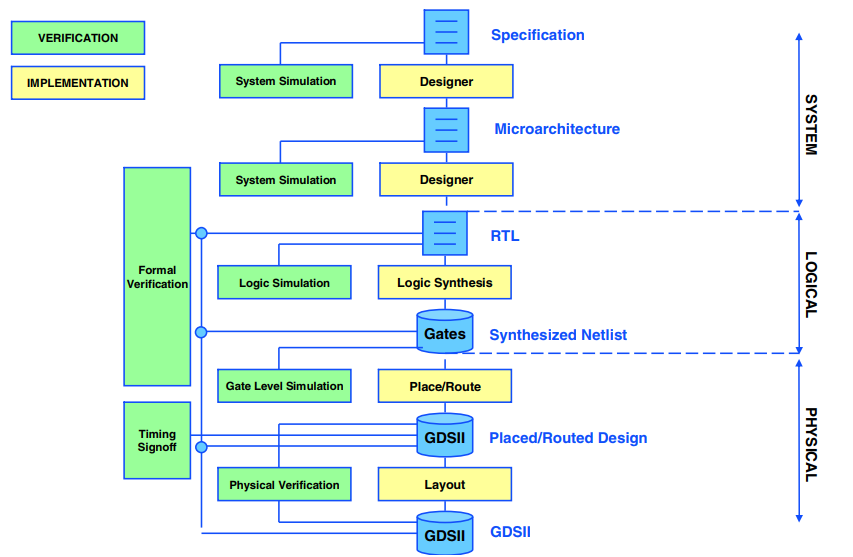
\includegraphics[width=\textwidth]{flow}
	\end{center}
\end{frame}
\subsection[Implementation]{Design Flow}
\begin{frame}
	\frametitle{Implementation Flow}
			\begin{columns}	
		\column{0.7\textwidth}
		\begin{center}
			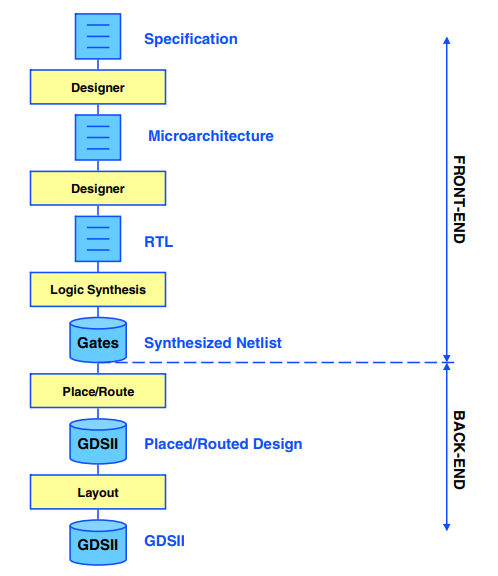
\includegraphics[width=0.7 \textwidth]{flow_2}
		\end{center}
		\column{0.5\textwidth}
		\begin{block}{Front-end}
			\textbf{Front-end chip design definition:}Processes in
			the overall chip design flow that involve system and logical design and verification
		\end{block}	
	\begin{block}{Back-end}
		\textbf{Back-end chip design definition}:Processes in the
		overall chip design flow that involve physical design and verification
	\end{block}	
	\end{columns}
\end{frame}
\subsection[Physical Design]{Back End or Physical Design}
\begin{frame}
	\frametitle{Implementation Flow}
The terms “physical design”or “back end”or “place/route”encompass many process steps, such as
	\begin{columns}	
		\column{1\textheight}
		\begin{itemize}
			\item Floorplanning
			\item Placement
			\item Clock Tree Synthesis (CTS)
			\item Route
			\item Extraction and Delay Calculation
			\item Static Timing Analysis (STA)
			\item EMIR
			\item Formal Verification
			\item Physical Verification
			\item Mask Prep 
		\end{itemize}
		\column{0.4\textheight}
		\begin{center}
			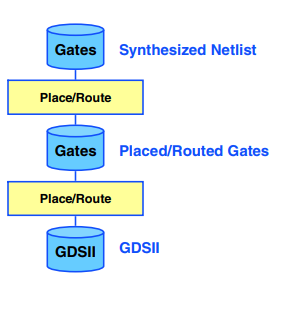
\includegraphics[width= 0.4\textheight]{simple}
		\end{center}
	\end{columns}
\end{frame}	
\begin{frame}
	\frametitle{Implementation Flow}
	\begin{center}
		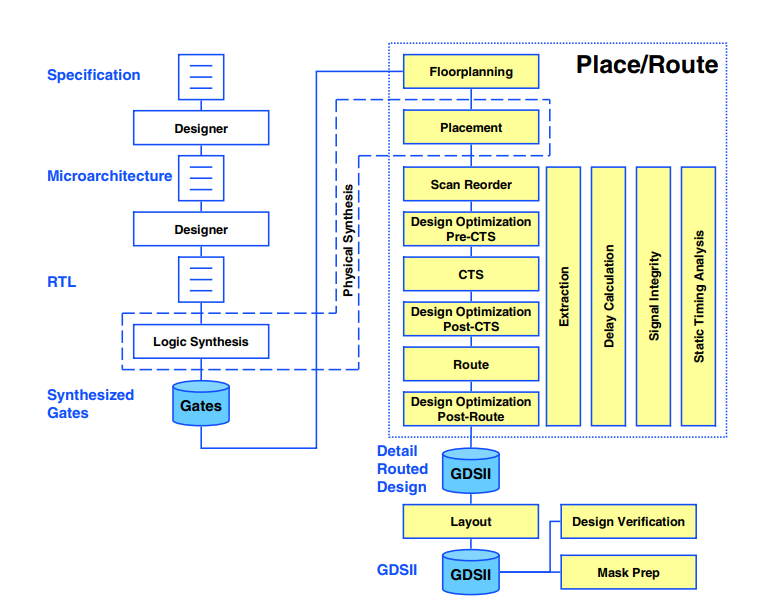
\includegraphics[width=0.8\textwidth]{PnR}
	\end{center}
\end{frame}	

\section[First]{First steps to design}
\subsection[Spec]{What Is a Specification}
\begin{frame}
	\frametitle{What Is a Specification?}
	\begin{columns}	
		\column{0.5\textwidth}
		Ideas begin with a specification, which can be a textual, graphical, or sometimes a software representation.
		\begin{itemize}
			\item \textbf{Definition:} A specification is an explicit set of requirements to be satisfied by a material, product,or service.
			\item \textbf{Example:} The specification for the latest chip specified a 250-MHz core clock with a serial interface, able to process 1 Mb of data per second at less than 10W total power.
		\end{itemize}
		\column{0.5\textwidth}
		\begin{center}
			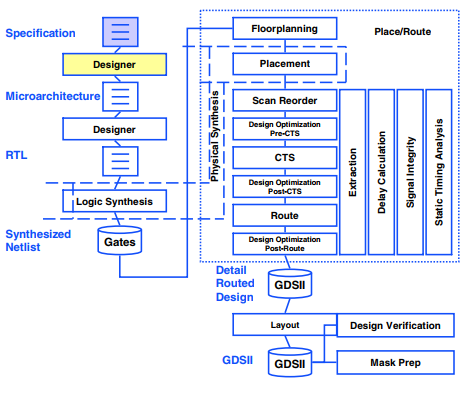
\includegraphics[width=\textwidth]{spec}
		\end{center}
	\end{columns}
\end{frame}
%-----------------------------------------
\begin{frame}
	\frametitle{Design Specification}
	\begin{columns}	
		\column{0.6\textwidth}
		\begin{block}{A list of requirements}
			\begin{itemize}
				\item \textbf{Function:}\newline
				What is expected
				from the ASIC 
				\item \textbf{Perfomance:}\newline What speed, power,
				area ?
				\item \textbf{I/O requirements:}\newline How will the ASIC fit
				together with the
				system ?
			\end{itemize}
		\end{block}
		
		\column{0.6\textwidth}
		\begin{center}
			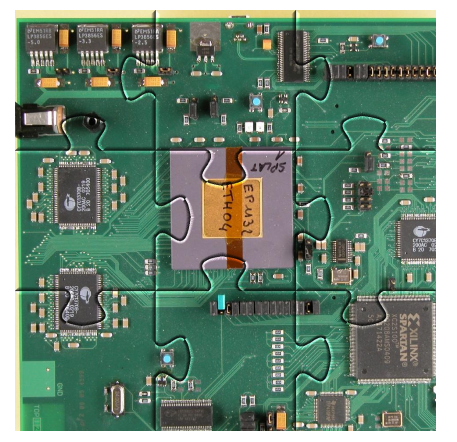
\includegraphics[width=0.8\textwidth]{chip}
		\end{center}
	\end{columns}
\end{frame}
%----------------------------------------------
\subsection[Feasibility ]{Is it possible to design the ASIC?}

\begin{frame}
\frametitle{We have specifications, but can we do it ?}
\begin{block}{Feasibility ?}
	For most of the projects:
	\begin{center}
		\textcolor{red}{\textbf{We have never done it, so we don’t know exactly!}}
	\end{center}
	We may:
	\begin{itemize}
		\item Have experience from earlier projects
		\item Make small experiments to estimate performance
		\item Choose appropriate technology
	\end{itemize}
\end{block}
	
\end{frame}

%-----------------------------------------
\subsection[Block]{Microarchitecture}
\begin{frame}
	\frametitle{What Is a Microarchitecture?}
	\begin{columns}	
		\column{0.5\textwidth}
		Step between the specification and
		RTL, the micro-architecture defines how
		the block will be implemented
		\begin{itemize}
			\item \textbf{Definition:} The microarchitecture
			implements the specification and
			defines specific mechanisms and
			structures for achieving that
			implementation
			\item \textbf{Example:} For Block A, the
			designer created a
			microarchitecture and partitioned
			the block into several smaller
			modules
		\end{itemize}
		\column{0.5\textwidth}
		\begin{center}
			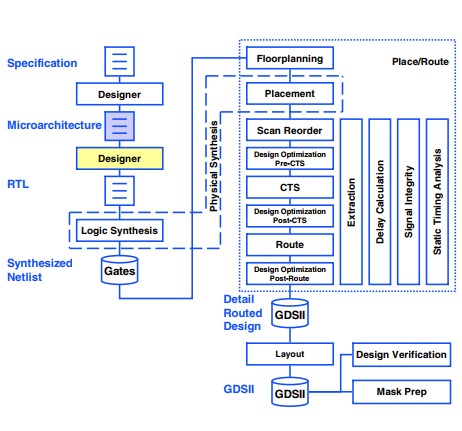
\includegraphics[width=\textwidth]{micro}
		\end{center}
	\end{columns}
\end{frame}
%----------------------------------------------------
\begin{frame}
	\frametitle{Always Start with a Block Diagram}
	\begin{columns}
		\column{0.5\textwidth}
		\begin{center}
			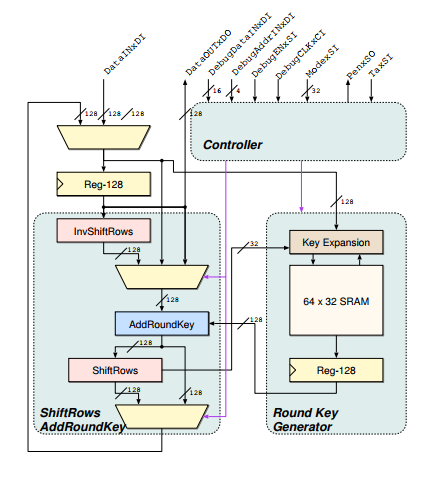
\includegraphics[width= \textwidth]{block_micro_arc}
		\end{center}	
		\column{0.5\textwidth}
		\begin{block}{Iterative Process}
			\begin{itemize}
				\item \textbf {Identify blocks} \newline
				What do we need to perform the functionality?
				\pause
				\item \textbf {Visualize structure} \newline
				How are blocks connected?
				\pause
				\item \textbf {Find critical paths} \newline
				Which block is most critical (speed, area, power)?
				\pause
				\item \textbf {Divide and Conquer} \newline
				Draw sub-block diagrams
			\end{itemize}
		\end{block}
	\end{columns}
\end{frame}
%---------------------------------------------------
\subsection[trans]{Architectural transformations}
\begin{frame}
	\frametitle{Architectural Transformations}
	\begin{columns}
		
		\column{0.5\textwidth}
		\begin{block}{Efficiency}
			Performance parameters:
			\begin{itemize}
				\item Area ($mm^{2}$)	
				\item Clock rate (MHz)
				\item Throughput(data/sec)
				\item Latency(num clock cycles)
			\end{itemize}
		\end{block}'
		\column{0.6\textwidth}
		\begin{center}
			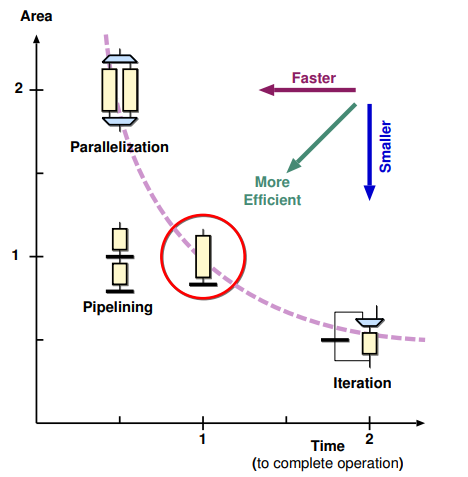
\includegraphics[width=0.9 \textwidth]{to_comp}
		\end{center}	
	\end{columns}
\end{frame}
%---------------------------------------------------
\begin{frame}
	\frametitle{Parallelization}
	\begin{columns}
		
		\column{0.5\textwidth}
		\begin{block}{More computation}
			If we use 2 parallel blocks:
			\begin{itemize}
				\item Area doubles
				\item Clock stays same
				\item Throughput doubles
				\item Latency stays same
			\end{itemize}
		\end{block}'
		\column{0.6\textwidth}
		\begin{center}
			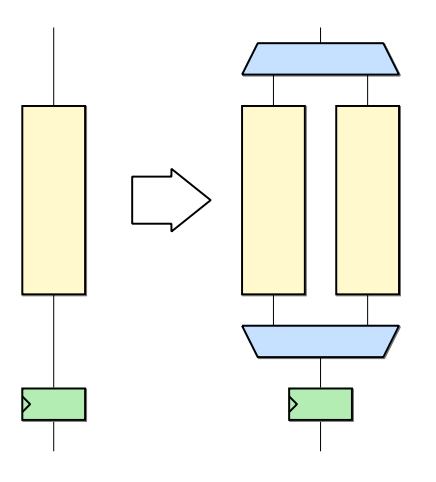
\includegraphics[width=0.7 \textwidth]{parallel}
		\end{center}	
	\end{columns}
\end{frame}

%---------------------------------------------------
\begin{frame}
	\frametitle{Pipelining}
	\begin{columns}
		
		\column{0.5\textwidth}
		\begin{block}{Faster computation}
			if we introduce one pipeline
			stage:
			\begin{itemize}
				\item Area increases a little
				\item Clock doubles
				\item Throughput doubles
				\item Latency doubles
			\end{itemize}
		\end{block}'
		\column{0.6\textwidth}
		\begin{center}
			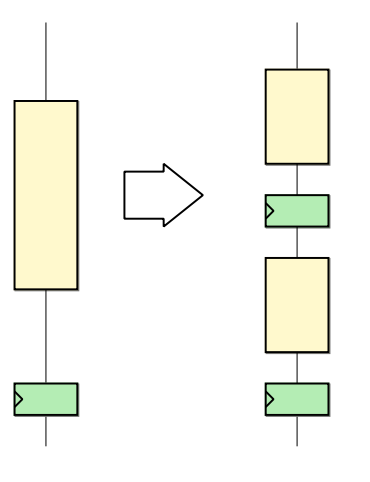
\includegraphics[width=0.7\textwidth]{pipe}
		\end{center}	
	\end{columns}
\end{frame}
%----------------------------------------------------
%----------------------------------------------------
\begin{frame}
	\frametitle{Iterative Decomposition}
	\begin{columns}
		
		\column{0.5\textwidth}
		\begin{block}{More clock cycles}
			If we can perform the
			operation in two iterations:
			\begin{itemize}
				\item Area halves
				\item Clock stays same
				\item Throughput halves
				\item Latency doubles
			\end{itemize}
		\end{block}'
		\column{0.6\textwidth}
		\begin{center}
			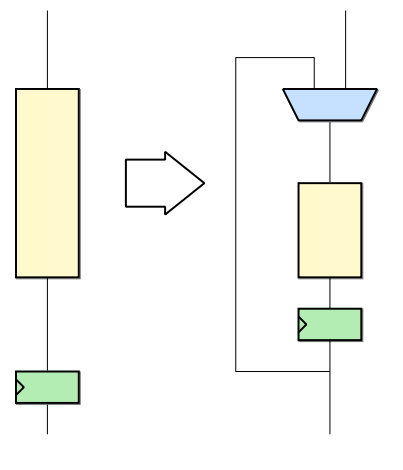
\includegraphics[width=0.7 \textwidth]{deco}
		\end{center}	
	\end{columns}
\end{frame}
%----------------------------------------------------
\begin{frame}
	\frametitle{Specification and Microarchitecture: Input and Output}
	\begin{columns}	
		\column{0.8\textwidth}
		\textbf{Specification}
		\begin{itemize}
			\item \textbf{Input:} Requirements from
			Marketing, CEO (Chief Executive
			Officer), CTO (Chief Technology
			Officer), etc
			\item \textbf{Output:} Document or model in
			text/graphics or software (C++,
			SystemC, SystemVerilog, etc.)
			format
		\end{itemize}
	\textbf{Microarchitecture}
	\begin{itemize}
		\item \textbf{Input:}  Specification + requirement from designer
		\item \textbf{Output:} Typically a document in
		text/graphics, could be software
		as well
	\end{itemize}
		\column{0.5\textwidth}
		\begin{center}
			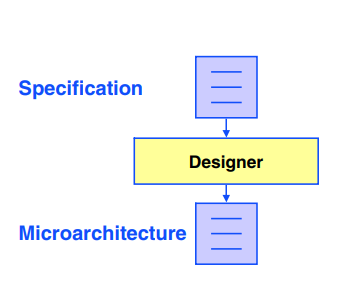
\includegraphics[width=0.6\textwidth]{spec_micro}
		\end{center}
	\end{columns}
\end{frame}
%----------------------------------------------------
\begin{frame}
	\frametitle{Example: Specification}
	\begin{columns}	
		\column{0.6\textwidth}
		Let’s assume we have a specification,
		microarchitecture, and RTL.
		\newline
		We are designing a chip called “EX”
		with
		\begin{itemize}
			\item Three main partitions “A,” “B,” and
			“C”
			\item Memories in each partition
			\item Perimeter I/O
			\item 250-MHz clock
			\item 10W total power
			\item Die size not to exceed 10x10 mm2
			due to custom package
			requirements
		\end{itemize}
		\column{0.5\textwidth}
		\begin{center}
			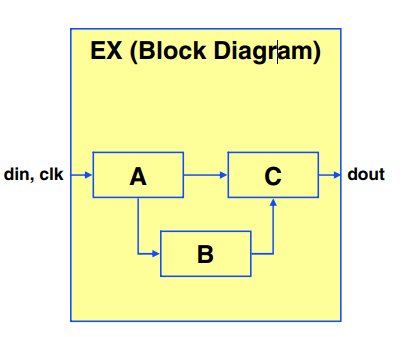
\includegraphics[width=0.9\textwidth]{block}
		\end{center}
	\end{columns}
\end{frame}
%-------------------------------------------
\begin{frame}
	\frametitle{Example: Microarchitecture}
	\begin{columns}	
		\column{0.6\textwidth}
		For Block C
		\begin{itemize}
			\item 32-bit data bus interface to
			Block A
			\item 16-bit control interface from
			Block B
			\item Use 64 Mb of SRAM
			\item Duplicate datapath elements in a
			parallel implementation
			\item Limit of five clock cycles from data
			input processed to data output
		\end{itemize}
		\column{0.5\textwidth}
		\begin{center}
			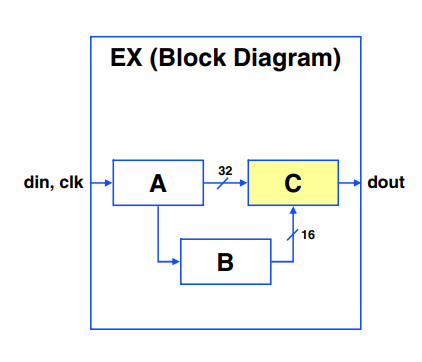
\includegraphics[width=0.9\textwidth]{block_micro}
		\end{center}
	\end{columns}
\end{frame}
%------------------------------------------------------
\section[Front]{Front-end}
\subsection[Modelling]{Modelling your design}
\begin{frame}
	\frametitle{Building a Model}
	\begin{block}{Make sure your system works}
		There are many languages that can be used for modelling:
		\begin{itemize}
			\item C, C++, SystemC
			\item Perl, Java, Tcl
			\item Matlab
			\item systemVerilog, Verilog, VHDL
		\end{itemize}
		\textcolor{red}{\textbf{This is not a religion, there is not one definitive answer.}} \newline
		Choose whatever is suitable, not always whatever you are
		comfortable with.
	\end{block}
\end{frame}

\begin{frame}
	\frametitle{Model Types}
	\begin{block}{Key words in modelling}
	There are many languages that can be used for modelling:
	\begin{itemize}
		\item \textbf {bit-true} \newline
		The model mimicks the hardware at bit level. Numbers are
		actually computed at the same accuracy as the hardware
		\item \textbf {cycle-true} \newline
		The model accurately replicates how the hardware works for
		every clock cycle.
		\item \textbf {transaction-based} \newline
		A high level model that works on blocks of data. It calculates
		the end result of the computation, intermediate steps are not
		available
	\end{itemize}
	\textcolor{red}{\textbf{The model is an important part of simulation environment}}
\end{block}
\end{frame}
%----------------------------------------
\subsection[HDL]{Describing hardware}
\begin{frame}
	\frametitle{Describing Hardware}
	\begin{columns}
		
		\column{0.5\textwidth}
		\begin{alertblock}{Next Lecture}
			We will discuss this topic
			in a second lecture
			\begin{itemize}
				\item How to turn an idea
				into an architecture
				\item How to come up with
				a block diagram
				\item Converting block
				diagram into Verilog, VHDL code
			\end{itemize}.
		\end{alertblock}
		\column{0.5\textwidth}
		\begin{center}
			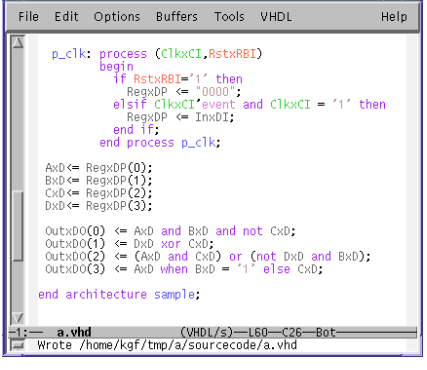
\includegraphics[width= \textwidth]{HDL}
		\end{center}	
	\end{columns}
\end{frame}
\subsection[Sim]{Simulating your Design}
\begin{frame}
	\frametitle{Simulating your Design}
	\begin{columns}
		\column{0.5\textwidth}
		\begin{center}
			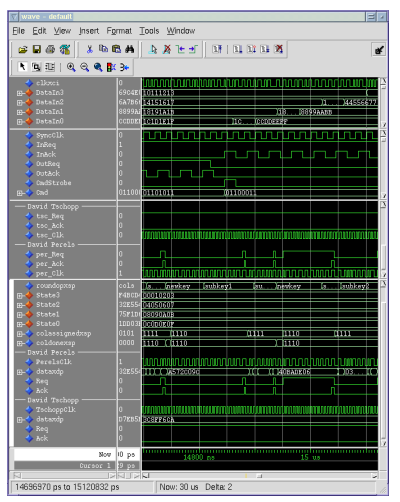
\includegraphics[width=\textwidth]{test}
		\end{center}
		
		\column{0.5\textwidth}
		\begin{block}{Does it actually work ?}
			\begin{itemize}
				\item \textbf {Behavioral simulation} \newline
				no delays for processing
				\item \textbf {No performance parameters} \newline
				only functionality is verified
				\item \textbf {Hardware description} \newline
				Not every construct in VHDL or Verilog can be implemented in hardware. This simulation will not show this.
			\end{itemize}.
		\end{block}
	\end{columns}
\end{frame}
%---------------------------------------------------
\subsection[Testb.]{Understanding testbenches}
\begin{frame}
	\frametitle{Testbenches}
	\begin{center}
		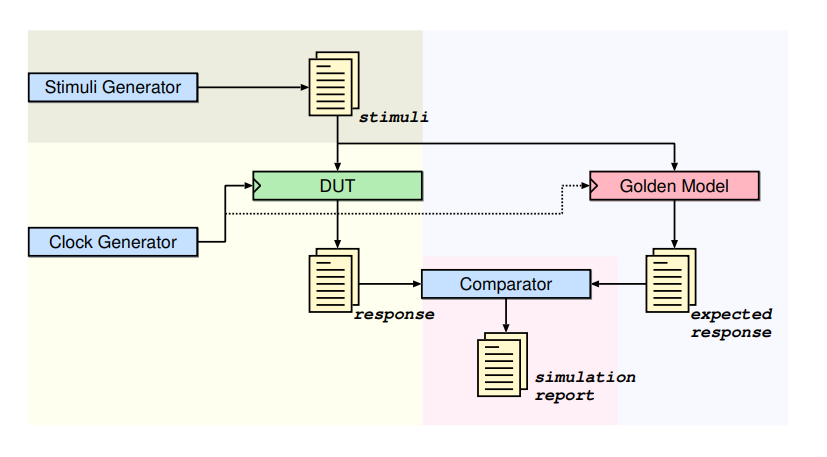
\includegraphics[width=\textwidth]{testb}
	\end{center}
\end{frame}
%----------------------------------------------
\subsection[Ver.]{Verification}
\begin{frame}
	\frametitle{Verification}
		\begin{block}{Bug hunting}
		\begin{itemize}
			\item \textbf {Time consuming} \newline
			The majority of design is verification
			\item \textbf {Exhaustive tests are not feasible} \newline
			A 32 bit adder has $2^{64}$ possible input combinations. If we
			check 1.000.000.000 inputs per second it will take 200 days !!
			\item \textbf {Every line we write, has a potential for error} \newline
			People talk about 1 bug every 20 lines of code.
			\item \textbf {Golden models can be wrong} \newline
			Sometimes, your hardware description is correct, but your
			model is wrong	
		\end{itemize}
	\end{block}
\end{frame}
%----------------------------------------------------
\subsection[Synth.]{Logic Synthesis}
\begin{frame}
	\frametitle{What Is Logic Synthesis?}
		\begin{columns}	
		\column{0.5\textwidth}
		\begin{itemize}
			\item \textbf{Definition:} The process of translating, optimizing, and mapping RTL code into a specified standard cell library.
			\item \textbf{Example:} To determine the feasibility of the design, we need to synthesize the RTL code into gates and measure timing, power, and area
		\end{itemize}
		\column{0.5\textwidth}
		\begin{center}
			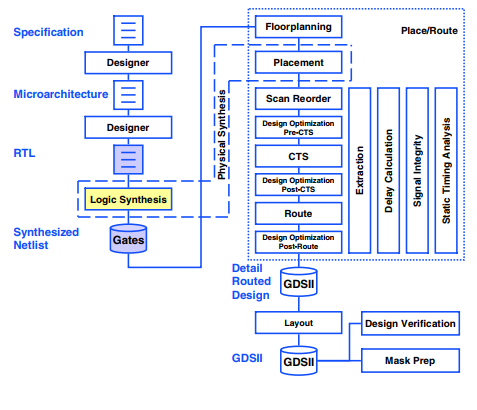
\includegraphics[width=\textwidth]{synthesis}
		\end{center}
	\end{columns}
\end{frame}
%----------------------------------------------
\begin{frame}
	\frametitle{Logic Synthesis Results}
		\begin{alertblock}{Synthesis is just a tool}
		\begin{itemize}
			\item Synthesis tools do not magically generate circuits
			\item They are supposed to generate exactly the circuit that you want
			\item You must have a good idea of what the synthesis result will be
			\pause
			\item If the result is not as you expect, you should convince the synthesizer to produce the correct result.
		\end{itemize}
	\end{alertblock}
\end{frame}
%----------------------------------------------
\begin{frame}
	\frametitle{Different constraints, different circuits}
	\begin{center}
		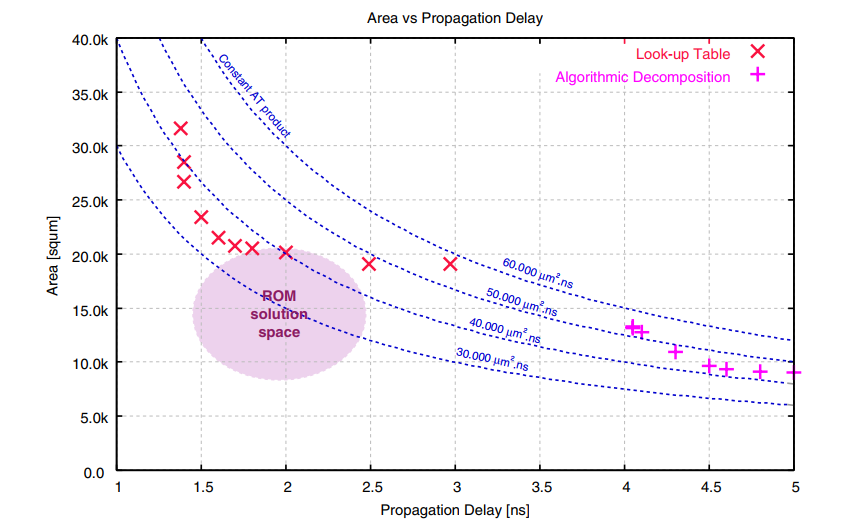
\includegraphics[width=\textwidth]{synth_1}
	\end{center}
\end{frame}
%----------------------------------------------
\begin{frame}
	\frametitle{Don’t trust the synthesizer too much}
	\begin{center}
		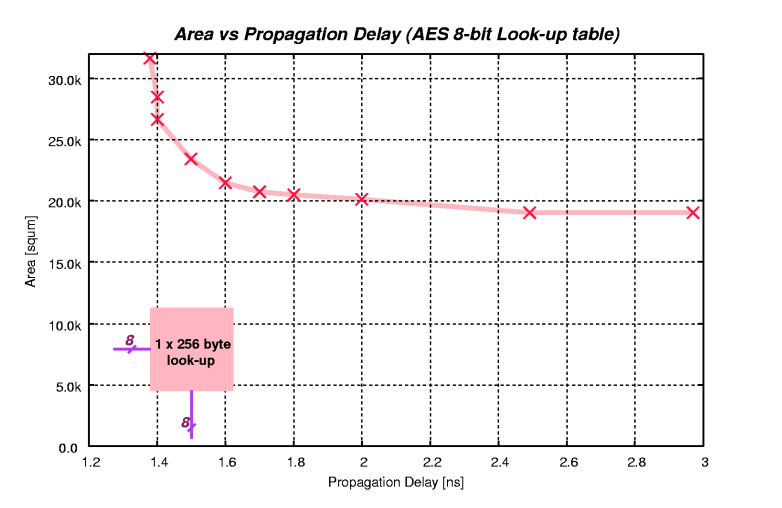
\includegraphics[width=\textwidth]{synthesizer1}
	\end{center}
\end{frame}
%----------------------------------------------
\begin{frame}
	\frametitle{Don’t trust the synthesizer too much}
	\begin{center}
		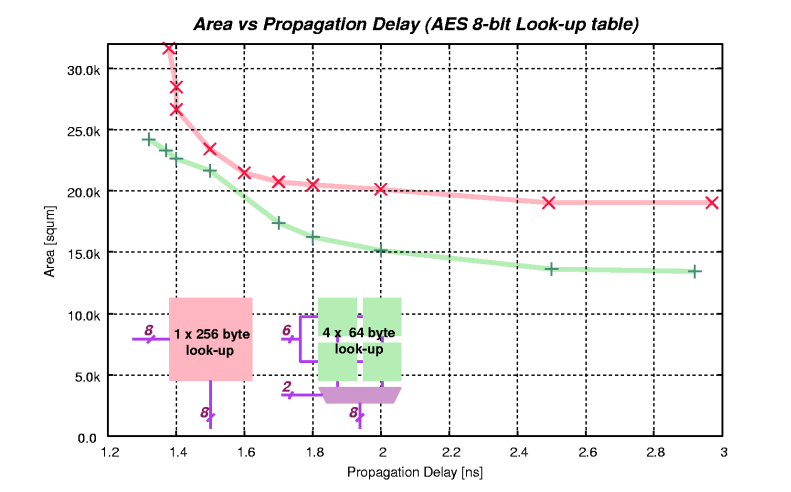
\includegraphics[width=\textwidth]{synthesizer2}
	\end{center}
\end{frame}
%----------------------------------------------
\begin{frame}
	\frametitle{Don’t trust the synthesizer too much}
	\begin{center}
		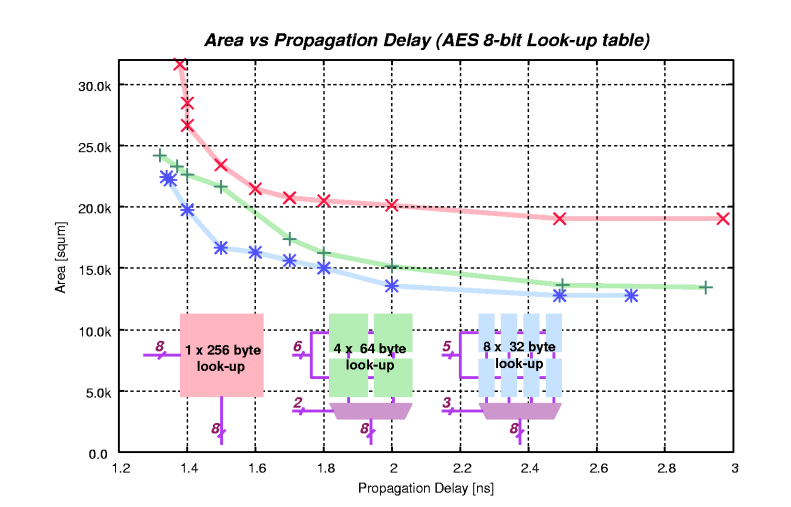
\includegraphics[width=\textwidth]{synthesizer3}
	\end{center}
\end{frame}
%----------------------------------------------
\begin{frame}
	\frametitle{Don’t trust the synthesizer too much}
	\begin{center}
		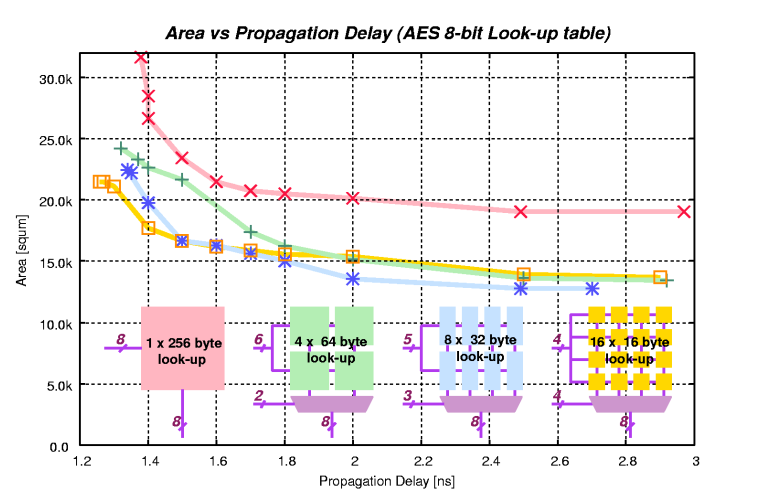
\includegraphics[width=\textwidth]{synthesizer4}
	\end{center}
\end{frame}
%----------------------------------------------
\begin{frame}
	\frametitle{Logic Synthesis: Input and Output}
		\begin{columns}	
		\column{0.5\textwidth}
		\begin{itemize}
			\item \textbf{Inputs:} 
			\begin{enumerate}
				\item RTL in the Verilog language or other HDL
				\item Constraints in Synopsys Design Constraints (SDC)
				\item Timing Libraries in Liberty (.lib)
			\end{enumerate}
			\item \textbf{Output:}
			\begin{enumerate}
				\item Gate Level Netlist(.v)
			\end{enumerate}
		\end{itemize}
		\column{0.5\textwidth}
		\begin{center}
			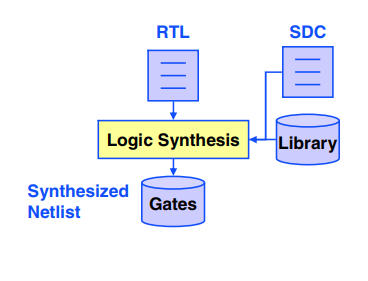
\includegraphics[width=0.8\textwidth]{inputs_outputs}
		\end{center}
	\end{columns}
\end{frame}
\begin{frame}
	\frametitle{Example: Logic Synthesis}
	Now that we have a working code, convert into hardware
	\begin{center}
		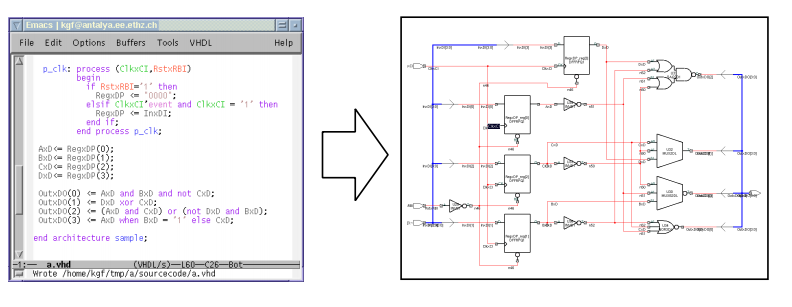
\includegraphics[width=\textwidth]{synth}
	\end{center}
\end{frame}		
%-------------------------------------------
\subsection[Cell]{Standard Cell Libraries}
\begin{frame}
	\frametitle{Standard Cell Libraries}
	\begin{columns}
		\column{0.5\textwidth}
		\begin{block}{Collection of pre-designed gates}
			\begin{itemize}
				\item \textbf {simple logic functions} \newline
				and, or, xor, not, nand, nor
				\item \textbf {complex logic functions} \newline
				adders, and-or-invert
				\item \textbf {sequential elements} \newline
				latches, flip-flops
				\item \textbf {different drive strengths} \newline
				Each cell has at least 2-4
				variations with different
				current driving capabilities	
			\end{itemize}.
		\end{block}
		\column{0.5\textwidth}
		\begin{center}
			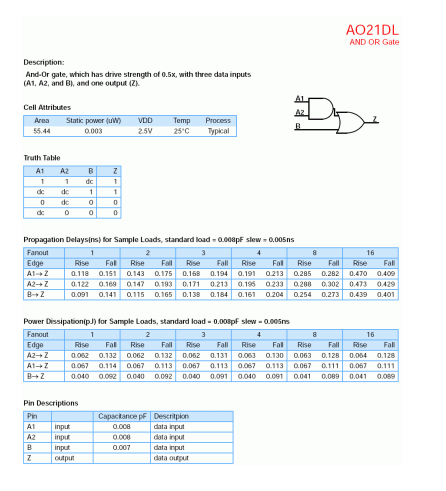
\includegraphics[width=\textwidth]{cells}
		\end{center}
	\end{columns}
\end{frame}
\begin{frame}
	\frametitle{Standard Cells - 2}
	\begin{center}
		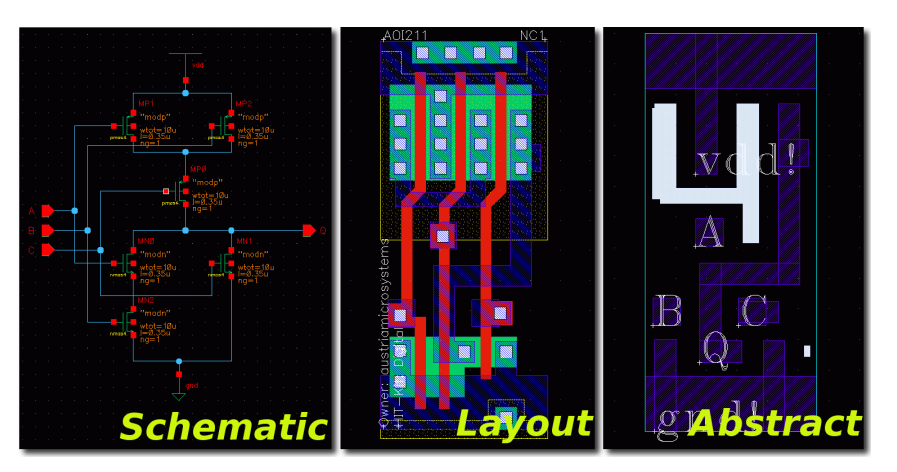
\includegraphics[width=\textwidth]{cell_2}
	\end{center}
\end{frame}
\begin{frame}
	\frametitle{Standard Cell Rows}
	\begin{center}
		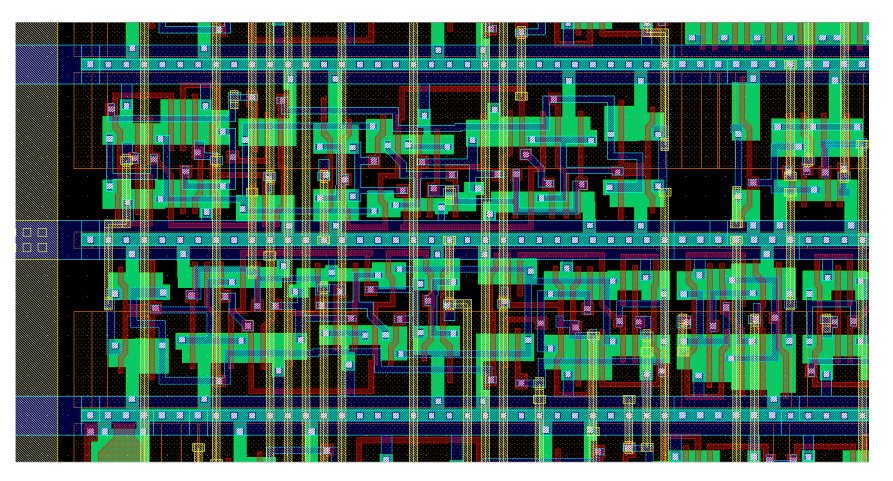
\includegraphics[width=\textwidth]{row}
	\end{center}
\end{frame}
%------------------------------------------------
%------------------------------------------------
\section[Back]{Back-end Design}
\subsection[Goals]{Netlist to Chip}
\begin{frame}
	\frametitle{Back-end Design}
		Now that we have a netlist, let us convert it to a physical layout
	\begin{center}
		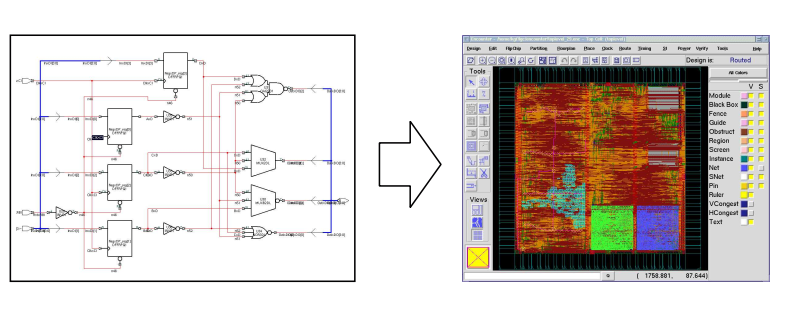
\includegraphics[width=\textwidth]{back}
	\end{center}
\end{frame}

%-----------------------------------------------
\subsection[Floor]{Floorplanning}
\begin{frame}
	\frametitle{What Is Floorplanning?}
	\begin{columns}
		\column{0.5\textwidth}
		\begin{itemize}
			\item \textbf {Definition:} Process of derivingthe die size, allocating space forsoft blocks, planning power, andmacro placement.
			\item \textbf {Example:} The three blocks of the chip were floorplanned to minimize the distance between the I/Os of the blocks and their
			interfaces to the chip. This
			reduces the routing between the
			blocks and, thus, improves the timing and routability of the design.
		\end{itemize}.
		\column{0.5\textwidth}
		\begin{center}
			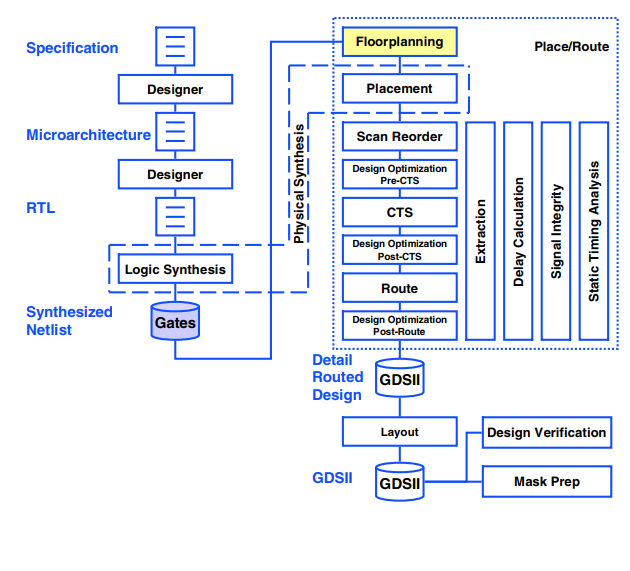
\includegraphics[width=\textwidth]{floor}
		\end{center}
	\end{columns}
\end{frame}
%--------------------------------------------
\begin{frame}
	\frametitle{Floorplanning: Input and Output}
	\begin{columns}
		\column{0.5\textwidth}	
		\begin{itemize}
			\item \textbf {Inputs:}
			\begin{enumerate}
				\item Gate Level Netlist
				\item Constraints in Synopsys Design Constraints (SDC)
				\item Logical Timing Libraries in Liberty (.lib)
				\item Physical Libraries in LEF format
				\item Floorplan constraints and script in TCL
			\end{enumerate}
			\item \textbf {Outputs:}
			\begin{enumerate}
				\item Floorplanned design in the Verilog language (logical connectivity data) or other HDL + DEF (physical data)
			\end{enumerate}	
		\end{itemize}
		\column{0.5\textwidth}
		\begin{center}
			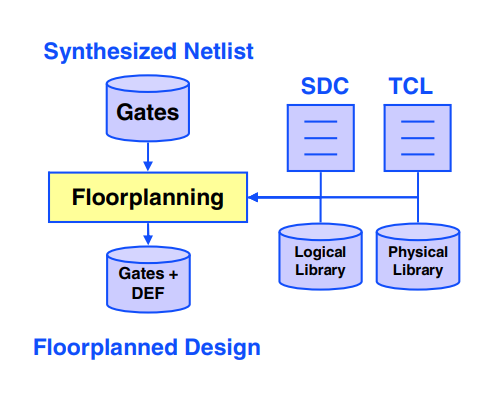
\includegraphics[width=\textwidth]{Fplan}
		\end{center}
	\end{columns}
\end{frame}
%-----------------------------------------------
\begin{frame}
	\frametitle{Floorplaning}
		\begin{columns}	
		\column{0.6\textwidth}
		\begin{center}
			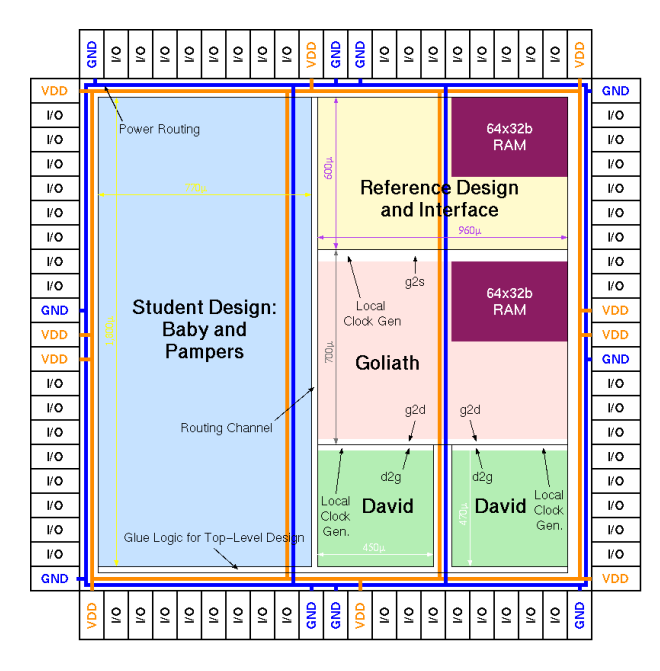
\includegraphics[width=\textwidth]{FChip}
		\end{center}
		
		\column{0.5\textwidth}
		\begin{block}{How will the chip look}
			\begin{itemize}
				\item Determine the total area/geometry of the chip
				\item Place the I/O cells
				\item Place pre-designed macro blocks 
				\item Leave room for routing, optimizations, power connections
				\pause
				\item \textcolor{red}{\textbf{iterative process}}, can not determine the perfect floorplan from the beginning
			\end{itemize}
		\end{block}
	\end{columns}
\end{frame}
%----------------------------------------------
\subsection[Power]{Power Planning}
\begin{frame}
	\frametitle{Power Planning}
	\begin{center}
		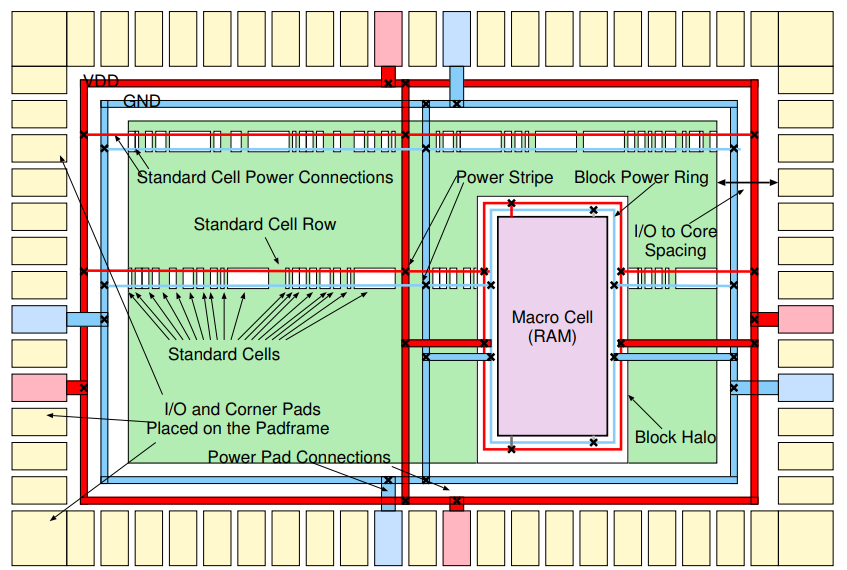
\includegraphics[width=\textwidth]{power}
	\end{center}
\end{frame}
%--------------------------------------------
\subsection[Place]{Placement}
\begin{frame}
	\frametitle{What Is Placement?}
	\begin{columns}
		\column{0.5\textwidth}
		\begin{itemize}
			\item \textbf {Definition:} Process of placing the standard cells in a floorplanned design.
			\item \textbf {Example:} After the chip was floorplanned, we performed placement and discovered the floorplan was too small to fit all of the cells and macros in the design.
			\item \textbf {Question:} How can we avoid this problem?
		\end{itemize}.
		\column{0.5\textwidth}
		\begin{center}
			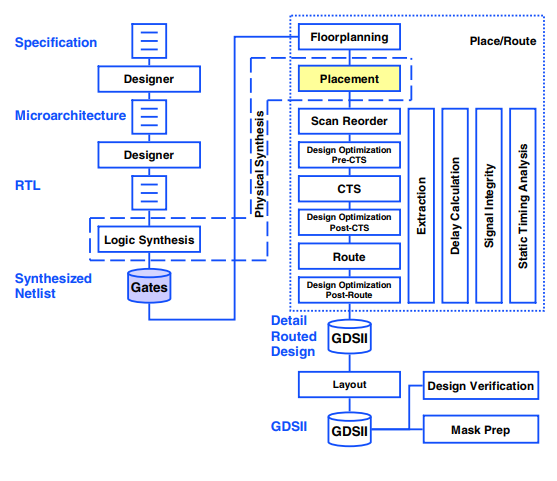
\includegraphics[width=\textwidth]{place}
		\end{center}
	\end{columns}
\end{frame}
%---------------------------------------------
\begin{frame}
	\frametitle{Placing Standard Cells}
	\begin{block}{NP hard problem}
		\begin{itemize}
			\item \textbf{Critical path is minimum}\newline
			Long interconnections on the critical path add capacitance
			\item \textbf{The design is routable}\newline
			Not all placements can be routed.
			\item \textbf{The area is minimum}\newline
			The routing overhead inreases area.
		\end{itemize}
	\end{block}
\end{frame}
%----------------------------------------------
\subsection[CTS]{Clock Tree Synthesis}
\begin{frame}
	\frametitle{What is Clock Tree Synthesis}
	\begin{columns}
		\column{0.5\textwidth}
		\begin{itemize}
			\item \textbf {Definition:} Process ofinserting buffers in the clockpath, with the goal ofminimizing clock skew andlatency to optimize timing
			\item \textbf {Example:} We ran clock treesynthesis on the exampleblock and saw a large clockskew due to bad clockconstraints.  We ended up re-running clock tree synthesiswith better constraints to getan optimal result.
		\end{itemize}.
		\column{0.5\textwidth}
		\begin{center}
			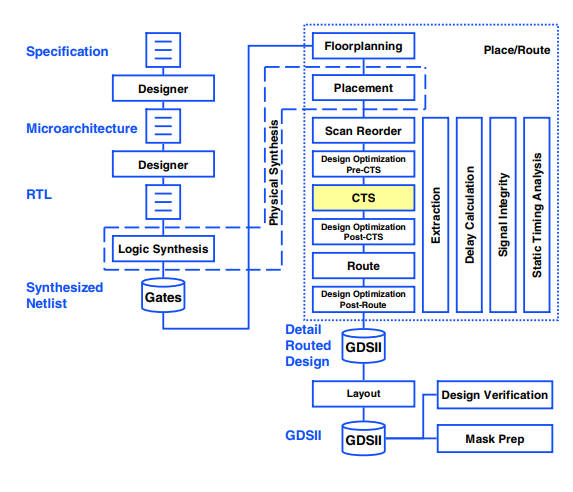
\includegraphics[width=\textwidth]{cts}
		\end{center}
	\end{columns}
\end{frame}
\begin{frame}
	\frametitle{Clock Distribution}
		\begin{block}{Clock is the most critical signal}
		\begin{itemize}
			\item Standard digital systems \textbf{rely} on the clock signal being present everywhere on the chip at the same time: \textcolor{red}{skew}
			\item Clock signal has to be connected to all flip-flops: \textcolor{red}{high fan out}
			\item Specialized tools insert multi level buffers (to drive the load) and balance the timing by ensuring the same wire length for all connection
			\pause
			\item The following example is a 200 MHz 3D image renderer with roughly 3 million transistors. The clock distribution has:
			\begin{enumerate}
				\item 10.928 flip-flops
				\item 9 level clock tree
				\item 478 buffers in the clock tree
				\item 34 cm total clock wiring
			\end{enumerate}
		\end{itemize}
	\end{block}
\end{frame}
\begin{frame}
	\begin{center}
		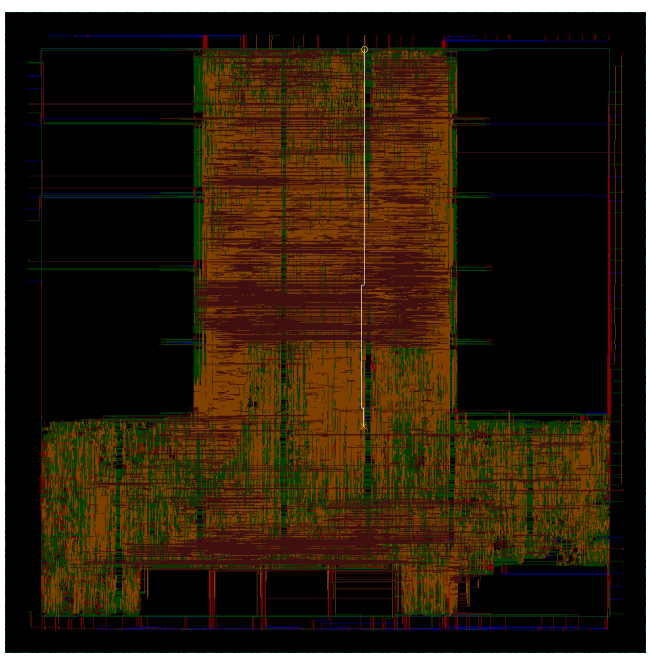
\includegraphics[width=0.7\textwidth]{clk}
	\end{center}
\end{frame}
\begin{frame}
	\begin{center}
		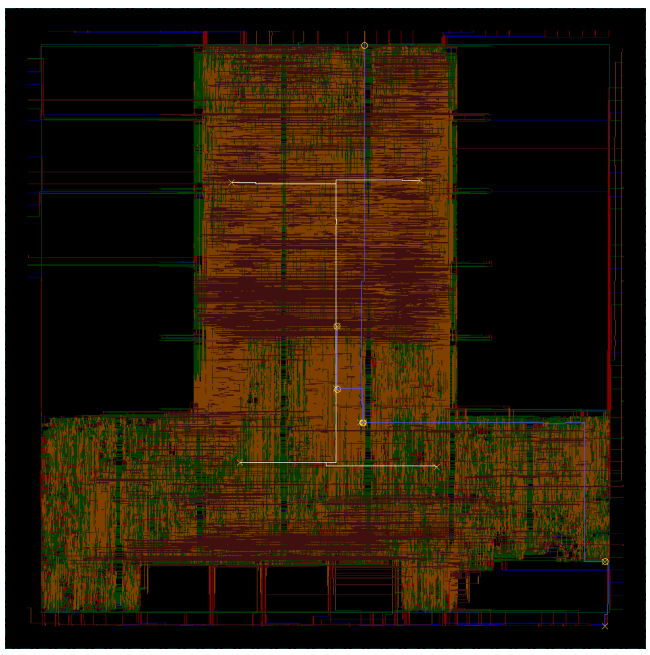
\includegraphics[width=0.7\textwidth]{clk2}
	\end{center}
\end{frame}
\begin{frame}
	\begin{center}
		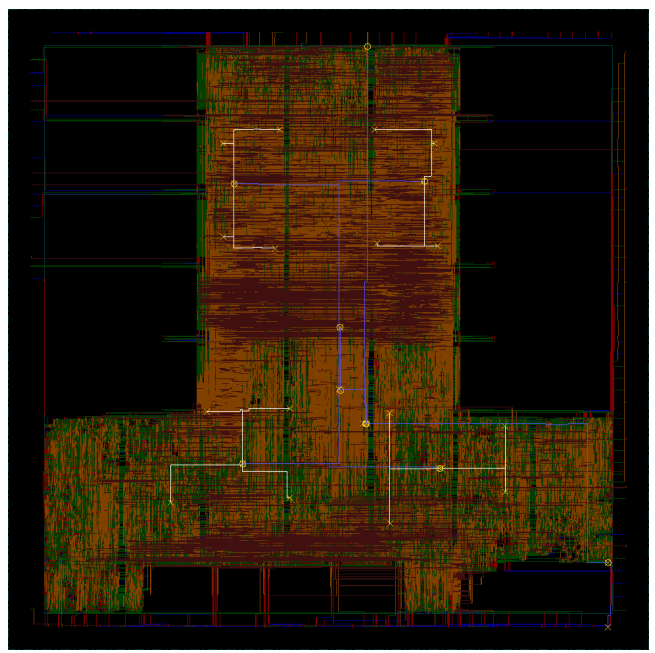
\includegraphics[width=0.7\textwidth]{clk3}
	\end{center}
\end{frame}
\begin{frame}
	\begin{center}
		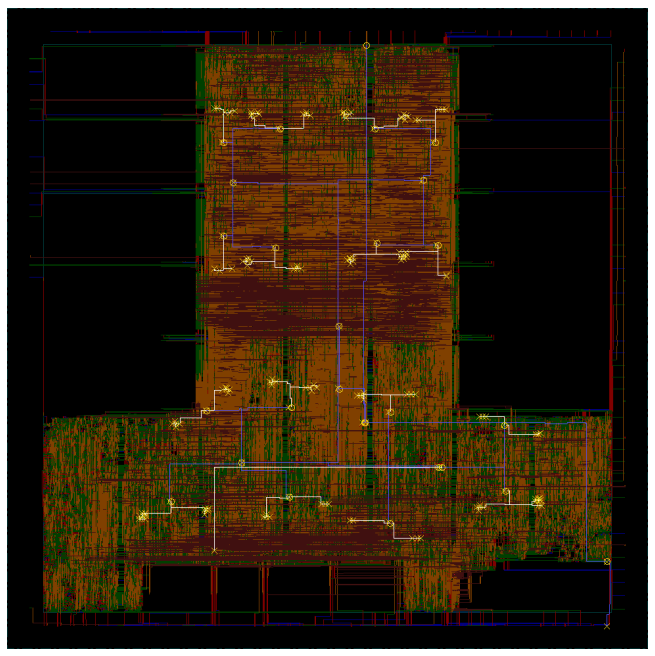
\includegraphics[width=0.7\textwidth]{clk4}
	\end{center}
\end{frame}
\begin{frame}
	\begin{center}
		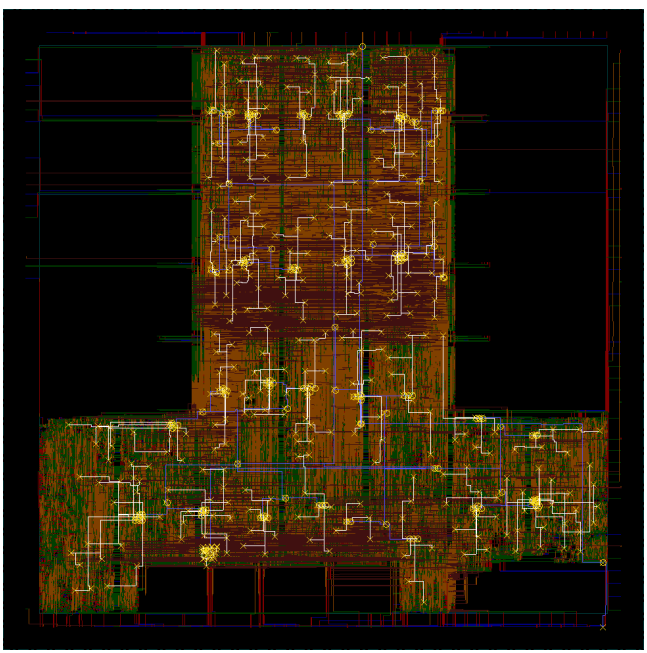
\includegraphics[width=0.7\textwidth]{clk5}
	\end{center}
\end{frame}
\begin{frame}
	\begin{center}
		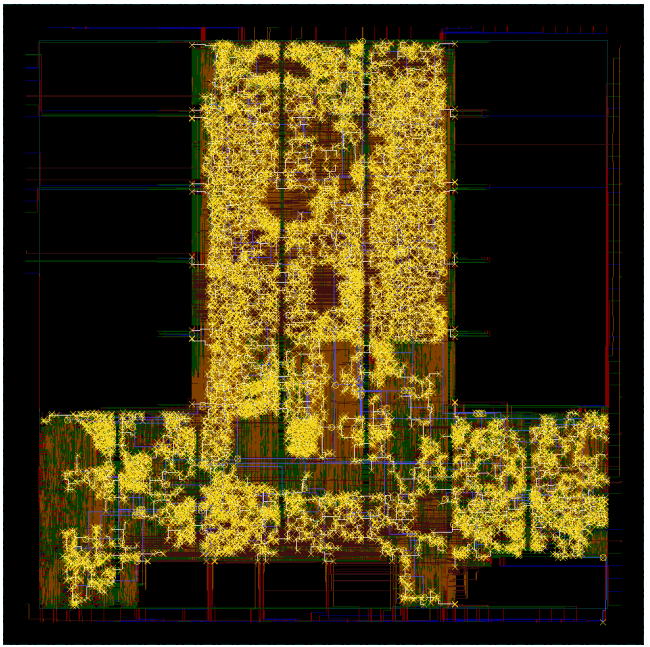
\includegraphics[width=0.7\textwidth]{clk6}
	\end{center}
\end{frame}
%---------------------------------------------
\subsection[Rout]{Routing}
\begin{frame}
	\frametitle{What Is Route?}
	\begin{columns}
		\column{0.6\textwidth}
		\begin{itemize}
			\item \textbf {Definition:} Process of
			connecting the pins of the
			standard cells, macros, and
			I/Os of a digital design to
			specific metal layers in the
			process technology to
			match the schematic
			\item \textbf {Example:} We ran a
			preliminary route on the
			example block and saw that
			routing congestion was an
			issue. To fix it, we re-ran
			placement with a placement
			density screen to force a
			lower utilization in that area
			and allow for more routing
			resources.
		\end{itemize}.
		\column{0.5\textwidth}
		\begin{center}
			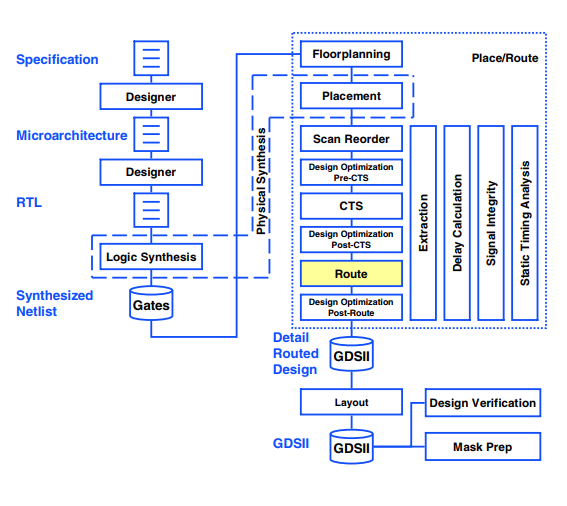
\includegraphics[width=\textwidth]{route}
		\end{center}
	\end{columns}
\end{frame}
\begin{frame}
	\frametitle{Routing}
	\begin{columns}	
		\column{0.5\textwidth}
		\begin{block}{Determine interconnection}
			\begin{itemize}
				\item Multiple (3-9) metal routing layers. Signals on different layers do not intersect.
				\item Vias to interconnect metals on adjacent layers.
				\item The longer the interconnection: 
				\begin{itemize}
					\item The more the capacitance
					\item The slower the connection
					\item The more the power consumption
				\end{itemize}
				\item Thin wires, vias add resistance
			\end{itemize}
		\end{block}
		\column{0.5\textwidth}
		\begin{center}
			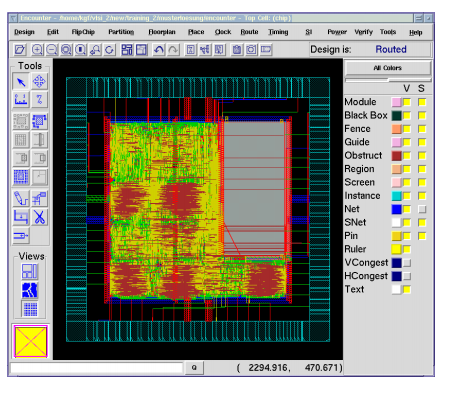
\includegraphics[width=\textwidth]{route2}
		\end{center}
	\end{columns}
\end{frame}
%------------------------------------------------
\subsection[Extr]{What Is Extraction?}
\begin{frame}
	\frametitle{Extraction}
\begin{columns}
	\column{0.6\textwidth}
	\begin{itemize}
		\item \textbf {Definition:} Process of calculating the parasitic resistance and capacitance of the interconnect of the physical design
		\item \textbf {Example:} Extraction can be performed at various parts of the design with varying accuracy. The most accurate results are achieved when extraction is performed on a fully routed design, because all of the nets are of known metal type and length. There are no 
	\end{itemize}.
	\column{0.5\textwidth}
	\begin{center}
		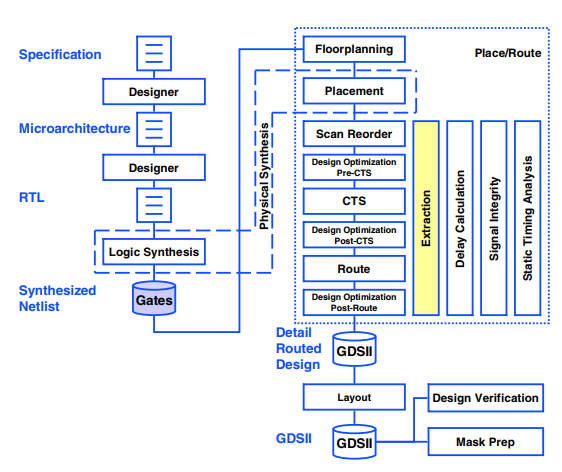
\includegraphics[width=\textwidth]{Extract}
	\end{center}
\end{columns}
\end{frame}
\begin{frame}
	\frametitle{Extraction}
		\begin{block}{Timing information depends on interconnect}
		Once the physical design is complete, everything about the
		interconnection network is known. It is possible to extract parasitic
		capacitance for the interconnection
		\begin{itemize}
			\item Wire capacitance
			\item Wire to wire capacitance
			\item Wire - via resistance
		\end{itemize}
		The extracted information can be used to extract timing
		information. It can be stored in special files (SDF, SPEF) and can
		be used by circuit simulators.
	\end{block}
\end{frame}
\subsection[Opt]{Optimization}
\begin{frame}
	\frametitle{Optimization}
	\begin{block}{Final timing with parasitics}
		Parasitics may influence timing severely. It is possible to make
		local optimizations to combat additional capacitance:
		\begin{itemize}
		\item Buffers are added to long connections
		\item Driver strength of the standard cells is adjusted
		\item Incremental change of placement
		\item Critical paths are resynthesized
	\end{itemize}
	\end{block}
\end{frame}
%----------------------------------------------
\section[PVR]{Physical Verification?}
\subsection[PVR]{Physical Verification?}
\begin{frame}
	\frametitle{What Is Design/Physical Verification?}
	\begin{columns}
		\column{0.8\textwidth}
		\begin{itemize}
			\item \textbf {Definition:} Layout versus schematic (LVS)and design rule check (DRC) and power (IR drop and EM) are signoff checks run to ensure the integrity, functionality, and manufacturability of the chip.
			\begin{itemize}
				\item LVS is a comparison of transistor-level SPICE netlist vs. GDSII to ensure the connectivity of the design.
				\item DRC is a detailed check of the physical design against the process technology rules.
				\item IR drop is a detailed check of the chip’s power plan to ensure that the supply voltages do not drop below accepted levels.
				\item  EM is a detailed check to ensure that the current density in all parts of the design does not exceed accepted levels.
			\end{itemize}.
		\end{itemize}
		\column{0.4\textwidth}
		\begin{center}
			\includegraphics[width=0.6\textwidth]{PVR}
		\end{center}
	\end{columns}
\end{frame}
%---------------------------------------------
\subsection[DRC]{DRC}
\begin{frame}
	\frametitle{DRC: Input and Output, Format}
	\begin{itemize}
		\item \textbf{Input}
			\begin{itemize}
			\item GDSII
			\item Rule deck
		\end{itemize}
		\item \textbf{Output}
		\begin{itemize}
		\item DRC reports
	\end{itemize}
	\end{itemize}
\begin{center}
	\includegraphics[width=0.5\textwidth]{DRC}
\end{center}
\end{frame}
\begin{frame}
	\frametitle{Design Rule Check}
	\begin{columns}	
		\column{0.5\textwidth}
		\begin{center}
			\includegraphics[width=\textwidth]{DRC_1}
		\end{center}
		\column{0.5\textwidth}
		\begin{block}{Production rules}
			Every physical layer has limits that are determined by the production flow. These include
			\begin{itemize}
				\item MMinimum spacing
				\item Minimum width
				\item Minimum coverage
				\item Minimum area
			\end{itemize}
		\end{block}
	\end{columns}
\end{frame}
%---------------------------------------------
\subsection[LVS]{LVS}
\begin{frame}
	\frametitle{LVS: Input and Output, Format}
	\begin{itemize}
		\item \textbf{Input}
		\begin{itemize}
			\item Gate Level Netlist
			\item GDSII
			\item Rule deck
			\item SPICE libraries
		\end{itemize}
		\item \textbf{Output}
		\begin{itemize}
			\item LVS reports
		\end{itemize}
	\end{itemize}
	\begin{center}
		\includegraphics[width=0.5\textwidth]{LVS}
	\end{center}
\end{frame}
\begin{frame}
	\frametitle{Layout Versus Schematic}

		\begin{block}{Is the layout equivalent to schematic}
			\begin{itemize}
				\item The physical layout contains only geometric information
				\item The devices (transistors) and interconnections are extracted.
				This is the extracted netlist
				\item The extracted netlist is compared to the initial netlist that we
				started with.
				\item Shorts between layers can be detected in this stage.
				\item \textcolor{red}{\textbf{Very important step}}, this step tells us that the chip is good
				to go.
			\end{itemize}
		\end{block}
\end{frame}
%---------------------------------------------
\subsection[EMIR]{EMIR}
\begin{frame}
	\frametitle{Power Grid Analysis, IR Drop, and EM: Input and Output}
	\begin{columns}	
		\column{0.6\textwidth}
		\begin{itemize}
			\item \textbf{Input}
			\begin{itemize}
				\item Gate Level Netlist + DEF
				\item Power characterized libraries in
				tool-specific 
				\item Timing libraries in Liberty (.lib)
				\item Timing constraints in SDC
				\item Extraction data in SPEF format
				\item Timing windows file (TWF)
				\item Value-change-dump file (optional)
			\end{itemize}
			\item \textbf{Output}
			\begin{itemize}
				\item IR drop reports
				\item EM reports
			\end{itemize}
			\end{itemize}
				\column{0.5\textwidth}
				\begin{center}
					\includegraphics[width=\textwidth]{EMIR}
				\end{center}
			\end{columns}
\end{frame}

\subsection[STA]{Static Time Analysis}
\begin{frame}
	\frametitle{Static Time Analysis Input and Output}
	\begin{columns}	
		\column{0.5\textwidth}
		\begin{itemize}
			\item \textbf{Input}
			\begin{itemize}
				\item Routed Gate Level Netlist  
				\item Timing libraries in Liberty (.lib)
				\item Timing constraints in SDC
				\item SPEF, SDF, and incremental SDF
				\item Timing windows file (TWF)
				\item Value-change-dump file (optional)
			\end{itemize}
			\item \textbf{Output}
			\begin{itemize}
				\item Timing reports, including noise-on-delay effects
			\end{itemize}
		\end{itemize}
		\column{0.5\textwidth}
		\begin{center}
			\includegraphics[width=\textwidth]{STA}
		\end{center}
	\end{columns}
\end{frame}
\subsection[Formality]{Formal Verification}
\begin{frame}
	\frametitle{Formal Verification Input and Output}
	\begin{columns}	
		\column{0.5\textwidth}
		\begin{itemize}
			\item \textbf{Input}
			\begin{itemize}
				\item Reference Design (RTL Code) 
				\item Implementation Design (Gate-Level Netlist)
				\item Setup Verification Format
			\end{itemize}
			\item \textbf{Output}
			\begin{itemize}
				\item Reports
			\end{itemize}
		\end{itemize}
		\column{0.5\textwidth}
		\begin{center}
			\includegraphics[width=\textwidth]{Formal}
		\end{center}
	\end{columns}
\end{frame}

\begin{frame}
	\frametitle{Chip is Finished, Now Time For Fun}
	\begin{center}
		\includegraphics[width=\textwidth]{chip_finish}
	\end{center}
\end{frame}
\subsection[Tape-out]{Tape-out}
\begin{frame}
	\frametitle{Tape-out}
	\begin{block}{Final stage of the design}
		\begin{itemize}
			\item In old times, the design data was transferred using magnetic
			tapes, hence the name
			\item The geometric data is electronically transfered to the
			production site
			\item Usually there will be an independent DRC check if problems
			are found, we get asked to correct the problems
			\item Then we \textcolor{red}{wait 10-14} weeks for production.
			\item Tape-out dates are well-known in advance, and are not
			negotiable. You \textcolor{red}{have to finish} by the given date, no mercy! 
		\end{itemize}
	\end{block}
\end{frame}
%----------------------------------------------
\section[Final]{Final Words}
\subsection[Chip]{Your own chip}
\begin{frame}
	\frametitle{Your Very Own Chip}
	\begin{center}
		\includegraphics[width=\textwidth]{chip_1}
	\end{center}
\end{frame}
\subsection[Testing]{Testing}
\begin{frame}
\frametitle{Testing}
\begin{block}{Now that we have our chip back}
	\begin{itemize}
		\item Does it really work ?
	\end{itemize}
	
\end{block}
\pause
\begin{center}
	\includegraphics[width=0.7\textwidth]{DFT}
\end{center}
\end{frame}
\subsection[Summary]{Summary of the Design Flow}
\begin{frame}
	\frametitle{Summary of the Design Flow}
	\begin{center}
		\includegraphics[width=0.7\textwidth]{summary}
	\end{center}
\end{frame}
\subsection[Nice]{A good looking chip will work good}
\begin{frame}
	\frametitle{A Good Looking Chip Will Always Work}
	\begin{center}
		\includegraphics[width=0.7\textwidth]{Final}
	\end{center}
\end{frame}
	\begin{frame}
	\frametitle{....}
	\begin{center}
		\<بِسْمِ اللَّـهِ الرَّحْمَـٰنِ الرَّحِيمِ> \\
		\<وَمَا أُوتِيتُمْ مِنَ الْعِلْمِ إِلَّا قَلِيلً>
		
	\end{center}
\end{frame}
%---------------------------------------------
\end{document} 